\documentclass[english,11pt]{beamer}

\DeclareMathOperator{\Cov}{Cov}
\DeclareMathOperator{\Var}{Var}
\DeclareMathOperator{\E}{\mathbb{E}}
\DeclareMathOperator{\Proba}{\mathbb{P}}

\newcommand{\Covb}[2]{\ensuremath{\Cov\!\left[#1,#2\right]}}
\newcommand{\Eb}[1]{\ensuremath{\E\!\left[#1\right]}}
\newcommand{\Pb}[1]{\ensuremath{\Proba\!\left[#1\right]}}
\newcommand{\Varb}[1]{\ensuremath{\Var\!\left[#1\right]}}

% norm
\newcommand{\norm}[1]{\| #1 \|}

\newcommand{\indep}{\rotatebox[origin=c]{90}{$\models$}}





\usepackage{mathptmx,amsmath,amssymb,graphicx,bibentry,bbm,babel,ragged2e}

\makeatletter

\newcommand{\noun}[1]{\textsc{#1}}
\newcommand{\jitem}[1]{\item \begin{justify} #1 \end{justify} \vfill{}}
\newcommand{\sframe}[2]{\frame{\frametitle{#1} #2}}

\newenvironment{centercolumns}{\begin{columns}[c]}{\end{columns}}
%\newenvironment{jitem}{\begin{justify}\begin{itemize}}{\end{itemize}\end{justify}}

\usetheme{Warsaw}
\setbeamertemplate{footline}[text line]{}
\setbeamercolor{structure}{fg=purple!50!blue, bg=purple!50!blue}

\setbeamersize{text margin left=15pt,text margin right=15pt}

\setbeamercovered{transparent}


\@ifundefined{showcaptionsetup}{}{%
 \PassOptionsToPackage{caption=false}{subfig}}
\usepackage{subfig}

\usepackage[utf8]{inputenc}
\usepackage[T1]{fontenc}



\makeatother

\begin{document}


\title{A Discrepancy-based Framework to Compare Robustness between Multi-Attribute Evaluations}

\author{J.~Raimbault$^{1,2}$\\
\texttt{juste.raimbault@parisgeo.cnrs.fr}
}


\institute{$^{1}$UMR CNRS 8504 G{\'e}ographie-cit{\'e}s\\
$^{2}$UMR-T IFSTTAR 9403 LVMT\\
}


\date{CSDM 2016 - Paris\\\smallskip
14th December 2016
}

\frame{\maketitle}


%%%
% Abstract

%Multi-objective evaluation is a necessary aspect when managing complex systems, as the intrinsic complexity of a system is generally closely linked to the potential number of optimization objectives. However, an evaluation makes no sense without its robustness being given (in the sense of its reliability). Statistical robustness computation methods are highly dependent of underlying statistical models. We propose a formulation of a model-independent framework in the case of integrated aggregated indicators (multi-attribute evaluation), that allows to define a relative measure of robustness taking into account data structure and indicator values. We implement and apply it to a synthetic case of urban systems based on Paris districts geography, and to real data for evaluation of income segregation for Greater Paris metropolitan area. First numerical results show the potentialities of this new method. Furthermore, its relative independence to system type and model may position it as an alternative to classical statistical robustness methods.
%\keywords{Multi-attribute Evaluation, Model-Independent Robustness, Urban System, Discrepancy}




%%%%%%%%%%%%%%%%%
\section{Introduction}
%%%%%%%%%%%%%%%%%

\subsection{Context}


\sframe{Multi-objective Complex Systems}{

% introduction with pictures/anecdote

\textit{From morphogenetic factors to optimal design, fundamental multi-objective nature of optimization processes}

\bigskip

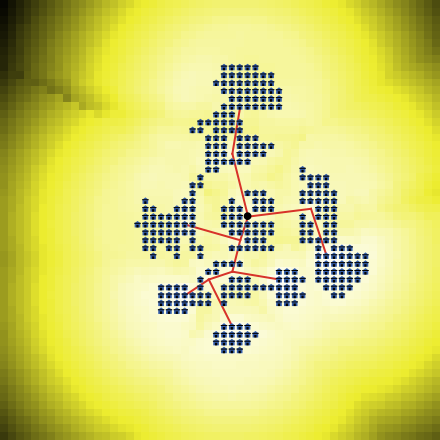
\includegraphics[width=0.35\textwidth]{figures/lattice}\hspace{0.5cm}
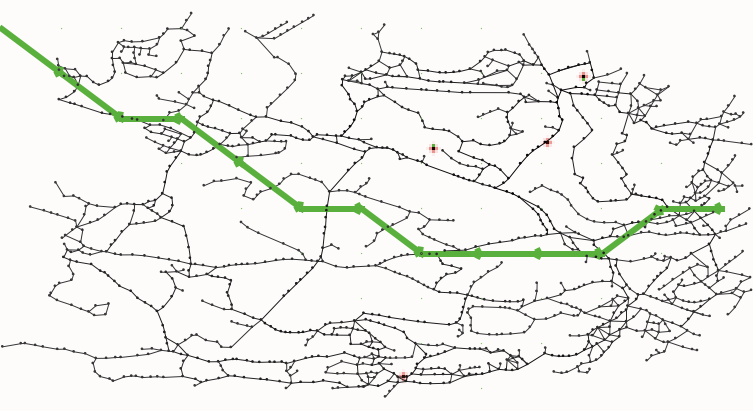
\includegraphics[width=0.55\textwidth]{figures/exampleOptimalCorridor}

\smallskip

{\footnotesize Source : Left \cite{raimbault2014hybrid} ; Right \cite{raimbault2015labex}}

}



\sframe{Multi-objective Evaluations of Socio-technical Systems}{

\justify

\textit{Systematic multi-objective nature of problems in design of Complex Industrial Systems~\cite{marler2004survey} and in the study of Complex Natural Systems~\cite{newman2011complex}}

\bigskip
\bigskip

$\rightarrow$ Design and understanding (i.e. evaluation) of Socio-technical systems at the intersection as hybrid systems~\cite{picon2013smart}\cite{haken2003face}

\bigskip

$\rightarrow$ Territorial systems as typical examples : e.g. sustainable urban design~\cite{souami2012ecoquartiers}, multi-criteria decision-making for transportation infrastructures~\cite{bavoux2005geographie}



}


\sframe{Robustness of Evaluations}{

\justify

\textit{Reliability of an evaluation is crucial; various approaches to robustness depending on method}

\bigskip
\bigskip

$\rightarrow$ Naturally included in the construction and estimation of statistical models~\cite{launer2014robustness} (e.g. p-value, beta power, AIC)

%\bigskip

%$\rightarrow$ Bayesian statistics also include robustness of sequential estimation

\bigskip

$\rightarrow$ In multi-objective optimization, diverse methods: sensitivity of Pareto front to perturbations~\cite{deb2006introducing};  continuity of solutions 

\cite{1688537}

\bigskip

$\rightarrow$ \cite{dobbie2013robustness} studies robustness for multi-attribute evaluations as biases depending on weighting techniques


}




\subsection{Research Question}


\sframe{Towards a Generic Robustness Framework}{

\justify

\textbf{Research Objective : } \textit{Investigate a generic data-driven approach to Robustness in Multi-attribute evaluations of Complex Socio-Technical Systems}

% put rationales here

% -> why multi -attribute
% -> data-driven
% -> model-independant

\bigskip
\bigskip

$\rightarrow$ Model-independence and method-independence; framework based only on data structure (and thus quality) and indicator values
\medskip

$\rightarrow$ Particular case of multi-attribute evaluations, where dimensions are aggregated, in order to obtain a simple measure of robustness

}


%%%%%%%%%%%%%%%%%
\section{Framework Description}
%%%%%%%%%%%%%%%%%




\subsection{Theoretical Framing}

\sframe{Intuitive and Theoretical Framing}{

% here theory is in the sense of thematic theory

\justify

\begin{enumerate}
\item {\justify Systems are seen from the perspective of raw data available: data-driven approach}

\smallskip

\item  A choice of indicators captures the realization of an ``urban fact''~\cite{mangin1999projet}, in the sense of stylized process with different spatial realizations

\smallskip

\item Given many systems and indicators, a common space can be build to compare them

\smallskip

\item Discrepancy of data~\cite{dick2010digital} in that space captures various aspects linked to robustness: system scale and range, precision of data, missing data 

\smallskip

\item Robustness must also capture an error done on indicator computation

\end{enumerate}

}





\subsection{Assumptions}


\sframe{Assumptions}{
\justify

% assumptions done

\textbf{Objectives as Kernel Integrals}

\medskip

$\rightarrow$ Kernel functions exist for each objective, computed as their integrals

\medskip

$\rightarrow$ Reasonable for most systems, as e.g. for territorial systems  it is analog to smoothing of Geographically Weighted Regression~\cite{brunsdon1998geographically}



\bigskip

\textbf{Linearly Aggregated Objectives}

\medskip

$\rightarrow$ Aggregated objective as linear combination of attributes $q(\vec{x})=\sum_i{w_i q_i(\vec{x})}$

\medskip

$\rightarrow$ Choice of weights at the core of decision-making process; not our scope here, we take simply relative indicator importance $w_{i,c}^{L}=\frac{\hat{q}_{i,c}}{\sum_{c}\hat{q}_{i,c}}$


}




\subsection{Formal Description}


\sframe{Formal Description (I)}{


\textbf{Territorial Systems : } Data $S_{i}=\mathbf{X}_{i}\in\mathcal{X}_{i}$ with $\mathcal{X}_{i}=\prod_{k}\mathcal{X}_{i,k}$ 

\medskip

\textbf{System space}

\[
\mathcal{X} \underset{def}{=} \left(\prod\tilde{\mathcal{X}}_{c}\right) = \left(\prod_{\mathcal{X}_{i,k}\in\mathcal{D}_{\mathcal{X}}}\mathbb{R}^{p_{i,k}^{X}}\right)
\]


\medskip

\textbf{Objectives :} $H_{c}$ space of real-valued functions on $\tilde{\mathcal{X}}_{c}$, such that :
\begin{enumerate}
\item $h_c\in H_{c}$ are ``enough'' regular (tempered distributions e.g.)
\item $q_c=\int_{\tilde{\mathcal{X}}_{c}}h$ is a function describing the ``urban fact'' (the indicator in itself)
\item Normalized kernels $h_c (\vec{x}) \in [0,1]$ % TYPO PAPER HERE ? not clear beween h_c and q_c ; both can be and are in applications
\end{enumerate}


}




\sframe{Formal Description (II)}{

Integral approximation theorem gives upper bound on error, linked to data discrepancy~\cite{niederreiter1972discrepancy}\cite{varet2010developpement}

\[
\left\Vert \int h_{c}-\frac{1}{n_{i,c}}\sum_{l}h_{c}(\vec{X}_{i,c,l})\right\Vert \leq K\cdot\left|\left|\left|h_{c}\right|\right|\right|\cdot D_{i,c}
\]

which propagates to the linear aggregation

\[
\left\Vert \int\sum w_{i,c}h_{c}-\frac{1}{n_{i,c}}\sum_{l}w_{i,c}h_{c}(\vec{X}_{i,c,l})\right\Vert \leq K\sum_{c}\left|w_{i,c}\right|\left|\left|\left|h_{c}\right|\right|\right|\cdot D_{i,c}
\]

\bigskip


$\rightarrow$ A relative \textit{Robustness Ratio} can thus be defined between two evaluations :

\begin{equation}
R_{i,i'}=\frac{\sum_{c}w_{i,c}\cdot D_{i,c}}{\sum_{c}w_{i',c}\cdot D_{i',c}}
\end{equation}


}






%%%%%%%%%%%%%%%%%
\section{Application}
%%%%%%%%%%%%%%%%%


\subsection{Synthetic Data}


\sframe{Implementation on Synthetic Data}{

% summary, data description, main result (summary of table)

\textit{Using OpenStreetMap roads and buildings data, construction of synthetic indicators on Paris districts (car daily use, car flows in streets, relative length of pedestrian streets), computed in Monte-carlo simulations}

\medskip

$\rightarrow$ Minimal ratio (relative to 1st Arr.) in 15th Arr. ($0.92 \pm 0.03$), intuitively expected

\bigskip

\centering


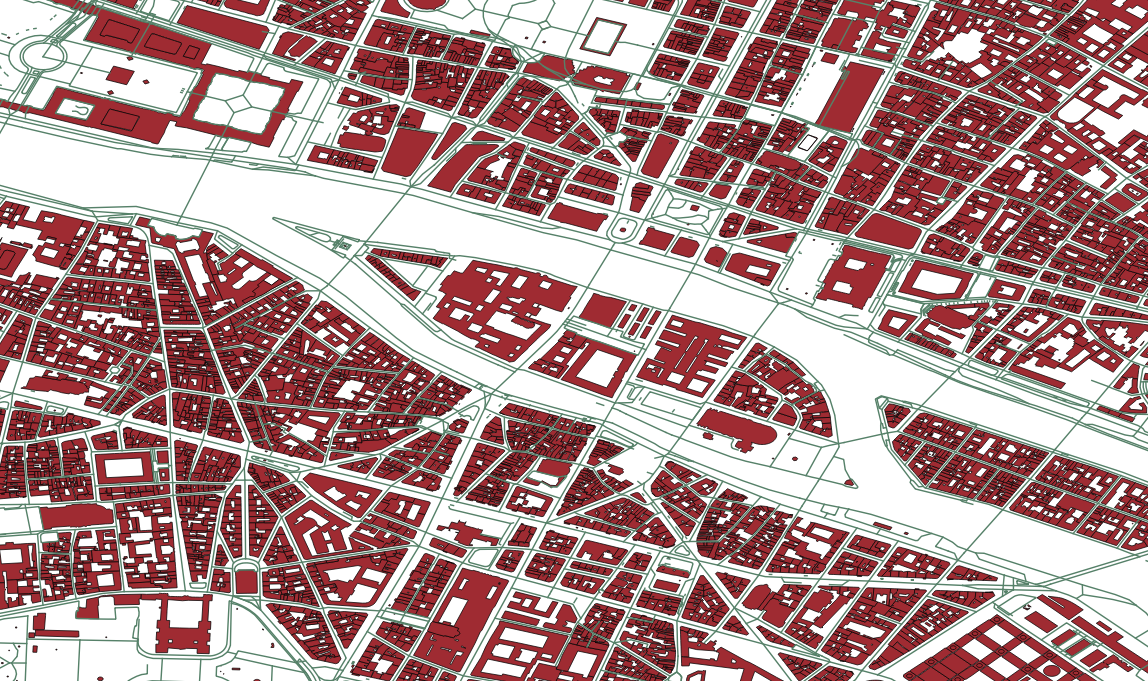
\includegraphics[width=0.5\textwidth]{figures/ex_data}

\smallskip

\small \textit{Example of raw data}

}


\subsection{Metropolitan Segregation}

\sframe{Metropolitan Segregation}{

% indicators, data

\textit{Application to metropolitan Segregation on Ile-de-France, Insee income data (2011)}

\bigskip
\bigskip

\textbf{Indicators : }

\begin{itemize}
\item Spatial autocorrelation Moran index
%defined as weighted normalized covariance of median income by $\rho = \frac{N}{\sum_{ij}w_{ij}}\cdot \frac{\sum_{ij}w_{ij}\left(X_i - \bar{X}\right)\left(X_j - \bar{X}\right)}{\sum_i \left(X_i - \bar{X}\right)^2}$
\item Dissimilarity index $d =  \frac{1}{\sum_{ij}w_{ij}} \sum_{ij} w_{ij} \left|\tilde{X}_i - \tilde{X}_j\right|$
%with $\tilde{X}_i = \frac{X_i - \min(X_k)}{\max(X_k) - \min(X_k)}$
\item Complementary of distribution entropy $\varepsilon = 1 + \frac{1}{\log(N)} \sum_i \frac{X_i}{\sum_k X_k} \cdot \log\left(\frac{X_i}{\sum_k X_k}\right)$
\end{itemize}

}

\sframe{Metropolitan Segregation: Indicators}{

% segreg maps

\textit{Example of Segregation maps (linking median income with local Moran index)}

\medskip

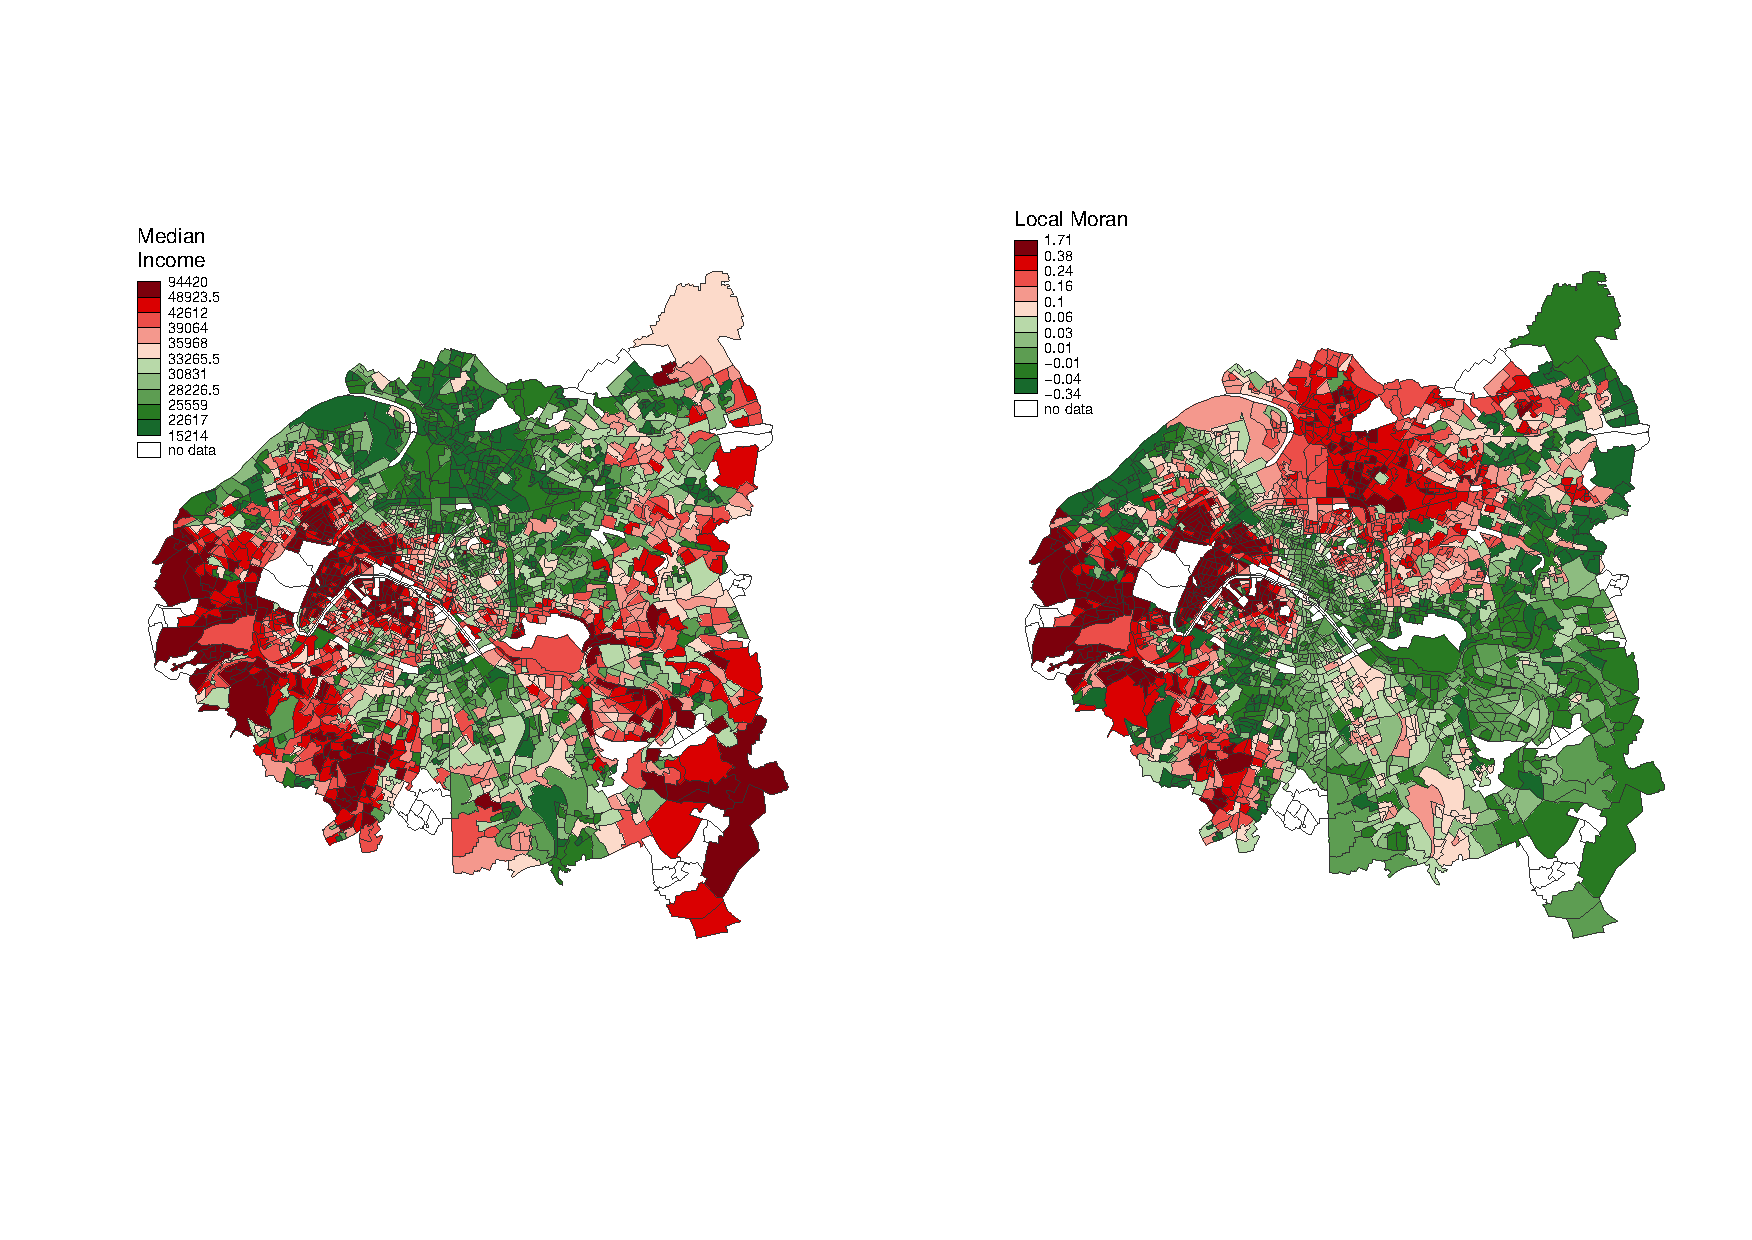
\includegraphics[width=\textwidth]{figures/grandParis_income_moran}


}


\sframe{Metropolitan Segregation: Results}{

% missing data
\textit{Framework Application : robustness comparison between administrative areas and sensitivity to missing data}

\bigskip

\centering

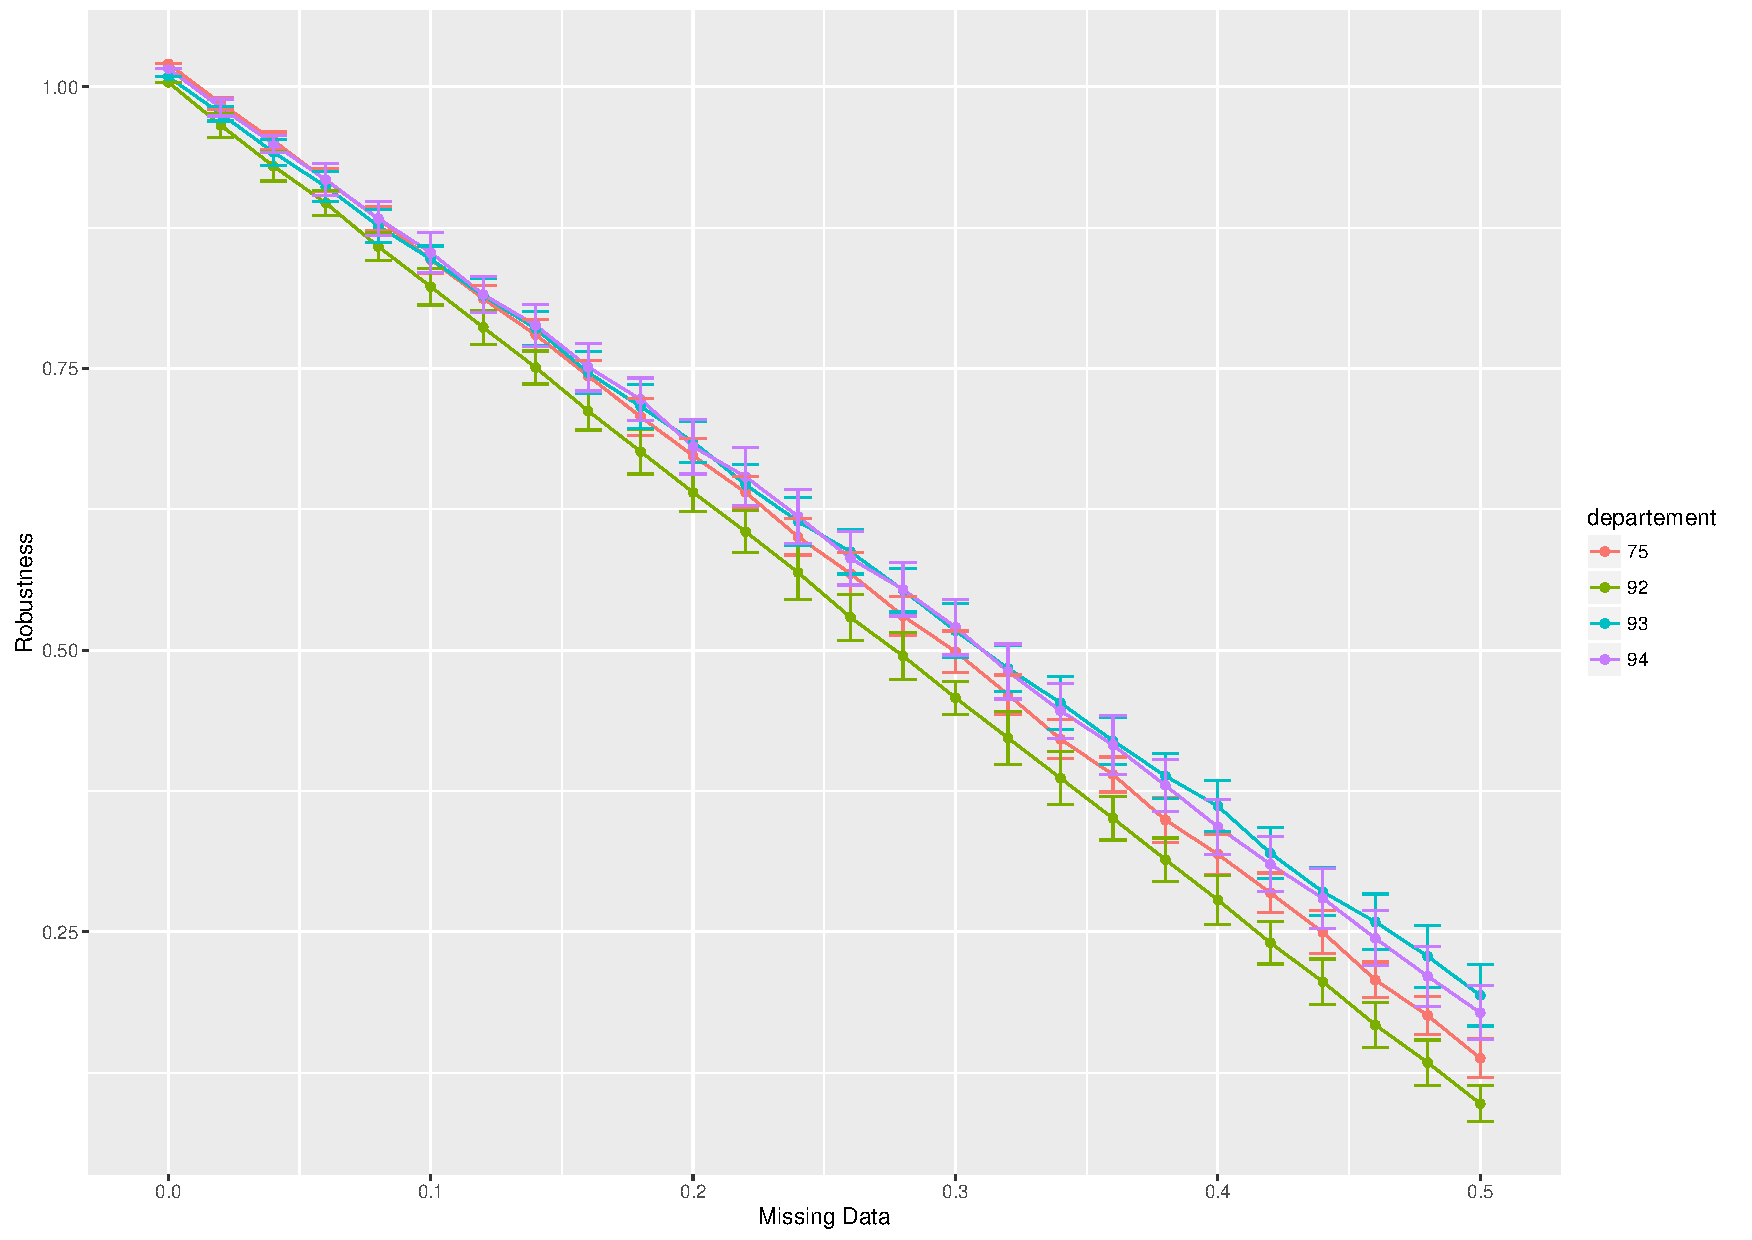
\includegraphics[width=0.55\textwidth]{figures/alldeps_rob_renormindics}
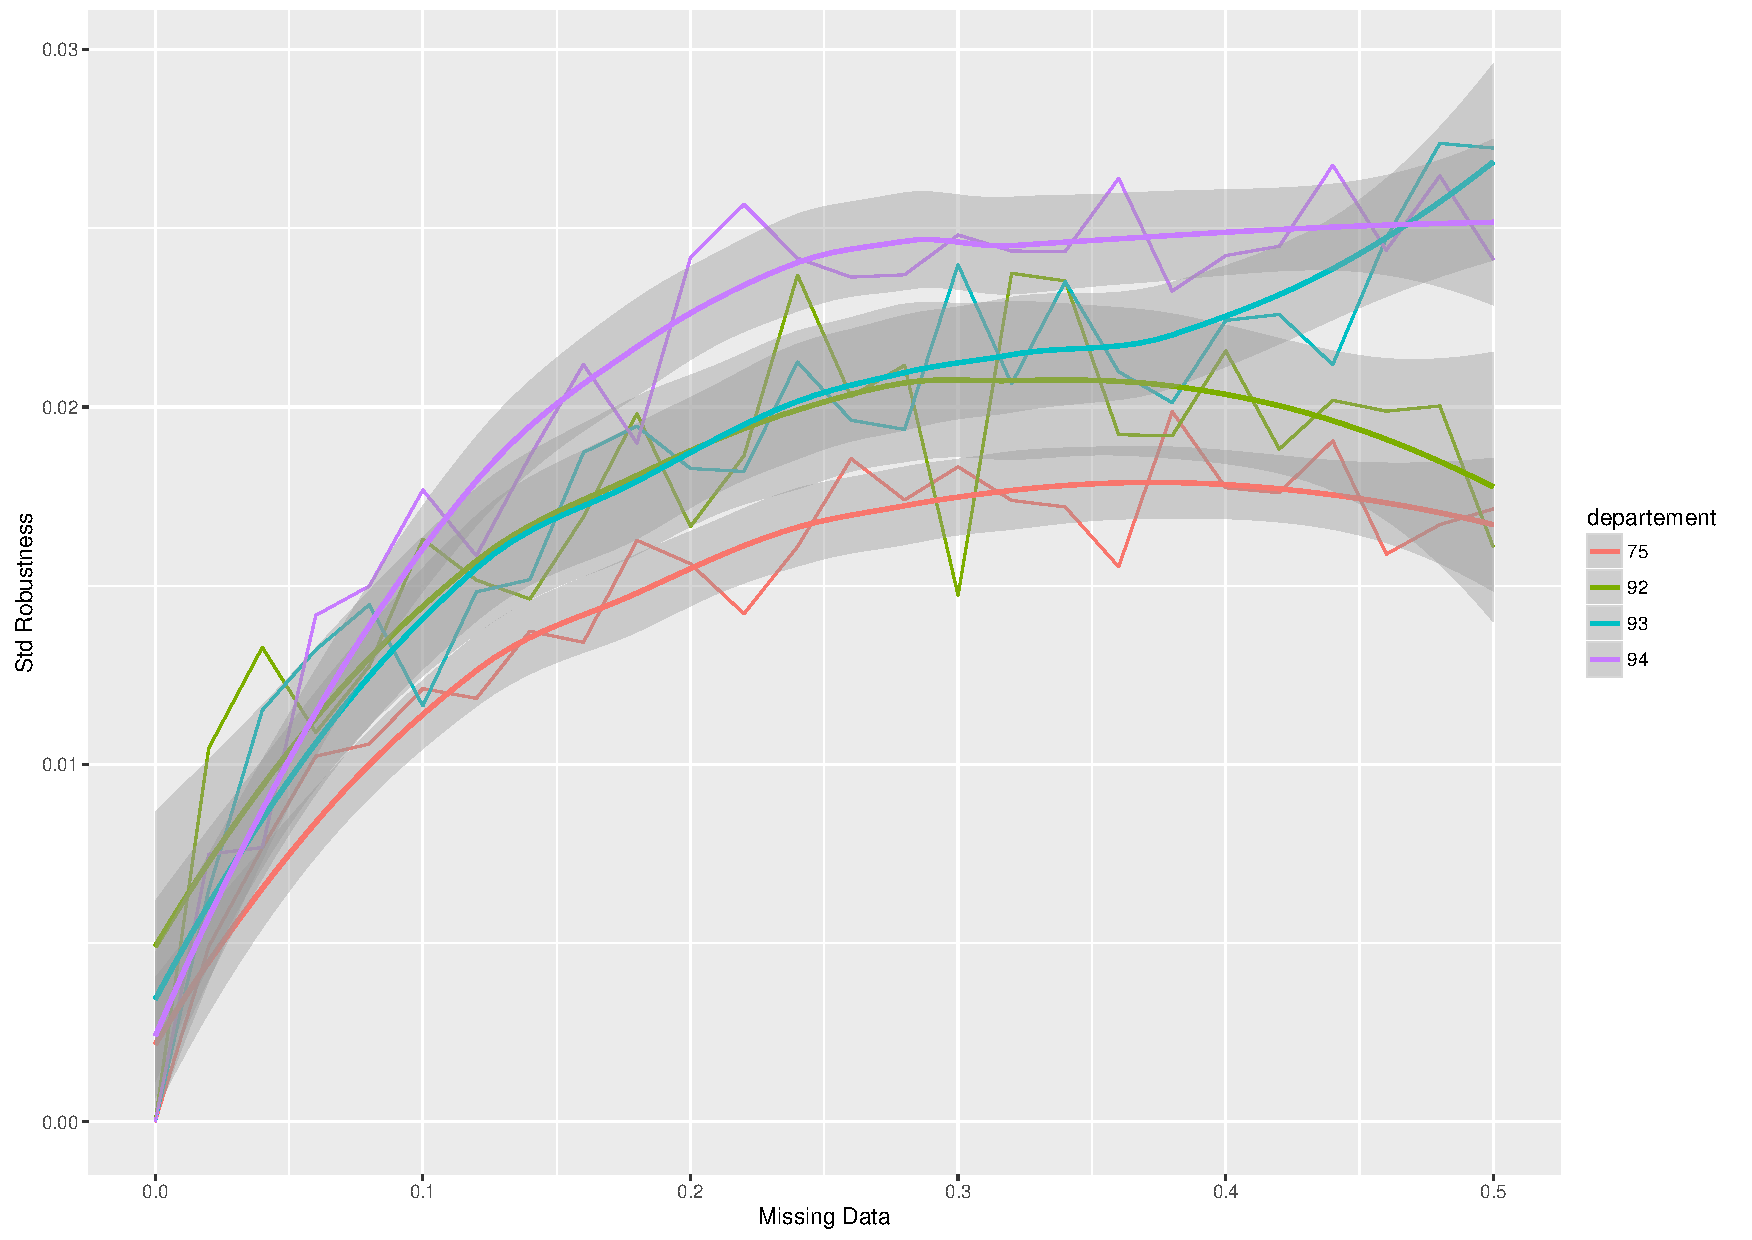
\includegraphics[width=0.55\textwidth]{figures/alldeps_robsd_renormindics}

% interpretation : different regimes.

\small \textit{(Left) Robustness ratio compared to full region for each area, as a function of missing data proportion; (Right) Standard deviations}

}



\subsection{Discussion}



\sframe{Discussion}{

\justify

\vspace{-0.5cm}

\textbf{Applicability}

\medskip

$\rightarrow$ Application to decision-making procedures : adding robustness as a dimension

\smallskip

$\rightarrow$ Assumptions validity ranges : some indicators may difficultly be viewed as spatial integrals (as some accessibility measures~\cite{kwan1998space})

\smallskip

$\rightarrow$ Availability of raw data


\bigskip

\textbf{Further Developments}

\medskip

$\rightarrow$ Application to existing open frameworks (e.g. \cite{tivadar2014oasis})

\smallskip

$\rightarrow$ More general formulation, first to non-linear aggregation (e.g. for Lipschitzian functions~\cite{dragomir1999ostrowski})

\smallskip

$\rightarrow$ Multi-dimensional measure of robustness using discrepancy along different dimensions



}




\sframe{Conclusion}{
\justify

$\rightarrow$ An original data-driven approach to robustness in multi-attribute evaluations of complex socio-technical systems; independent of model and method

\medskip

$\rightarrow$ Future insights from application to diverse system types and fields should refine the framework

\medskip

$\rightarrow$ Importance of interdisciplinarity (linking here statistics with computational modeling), crucial to study Complex Systems



\bigskip


\footnotesize{ 

- Special thanks to J. Keutchayan (Ecole Polytechnique de Montr{\'e}al) for suggesting the original idea of using discrepancy

\medskip

- All code and data available at \texttt{https://github.com/JusteRaimbault/RobustnessDiscrepancy}

\medskip

 - Paper preprint available \cite{raimbault2016discrepancy} at \texttt{http://arxiv.org/abs/1608.00840}
}

}




\sframe{Reserve Slides}{

\centering

\Large \textbf{Reserve Slides}


}




\sframe{Kernel Examples}{

Typical concrete example of kernels can be :

\begin{itemize}
\item A mean of rows of $\mathbf{X}_{i,c}$ is computed with $h(x)=x\cdot f_{i,c}(x)$ where $f_{i,c}$ is the density of the distribution of the assumed underlying variable.
\item A rate of elements respecting a given condition $C$, $h(x)=f_{i,c}(x)\chi_{C(x)}$ 
\item For already aggregated variables $\mathbf{Y}$, a Dirac distribution allows to express them also as a kernel integral. 
\end{itemize}

}


\sframe{Implementation}{

\begin{itemize}
\item Preprocessing of geographical data is made through QGIS 

\cite{qgis2011quantum}
\item Core implementation of the framework is done in R \cite{team2000r} for the flexibility of data management and statistical computations 
\item package \texttt{DiceDesign}\cite{franco20092} for computation of discrepancies
\end{itemize}

}



\sframe{Synthetic Indicators (I)}{
\begin{itemize}
\item Complementary of the average daily distance to work with car per individual, approximated by, with $n_{cars}(b)$ number of cars in the building (randomly generated by associated of cars to a number of building proportional to motorization rate $\alpha_m ~ 0.4$ in Paris), $d_w$ distance to work of individuals (generated from the building to a uniformly generated random point in spatial extent of the dataset), and $d_{max}$ the diameter of Paris area, $\bar{d}_w = 1 - \frac{1}{|b\in A(a)|} \cdot \sum_{b\in A(a)}{n_{cars}(b)\cdot \frac{d_w}{d_{max}}}$

\end{itemize}


}

\sframe{Synthetic Indicators (II)}{

\begin{itemize}
\item Complementary of average car flows within the streets in the district, approximated by, with $\varphi(s)$ relative flow in street segment $s$, generated through the minimum of 1 and a log-normal distribution adjusted to have $95\%$ of mass smaller than 1 what mimics the hierarchical distribution of street use (corresponding to betweenness centrality), and $l(s)$ segment length, $\bar{\varphi} = 1 - \frac{1}{|s\in A(a)|} \cdot \sum_{s \in A(a)}{\varphi(s)\cdot \frac{l(s)}{\max{(l(s))}}}$
\item Relative length of pedestrian streets $\bar{p}$, computed through a randomly uniformly generated dummy variable adjusted to have a fixed global proportion of segments that are pedestrian.
\end{itemize}
}

\begin{frame}
\frametitle{Synthetic Numerical Results}

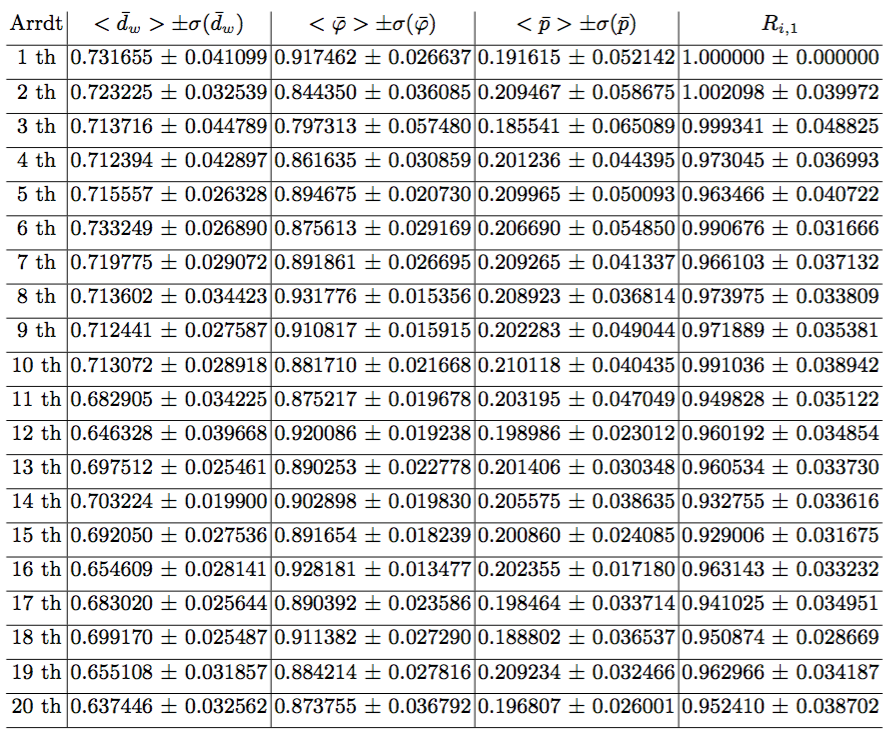
\includegraphics[width=\textwidth,height=0.9\textheight]{figures/syntheticnum.png}

\end{frame}




%%%%%%%%%%%%%%%%%%%%%
\begin{frame}[allowframebreaks]
\frametitle{References}
\bibliographystyle{apalike}
\bibliography{/Users/Juste/Documents/ComplexSystems/CityNetwork/Biblio/Bibtex/CityNetwork,biblio}
\end{frame}
%%%%%%%%%%%%%%%%%%%%%%%%%%%%












\end{document}







